\section{Integration of Concepts}
\textcolor{red}{What happens here is to bring the simulated data into a format that is compatible with my analysis of the real-life events data.}
 \begin{figure}[!ht]
	\begin{center}
		\makebox[\textwidth]{
			\centering
			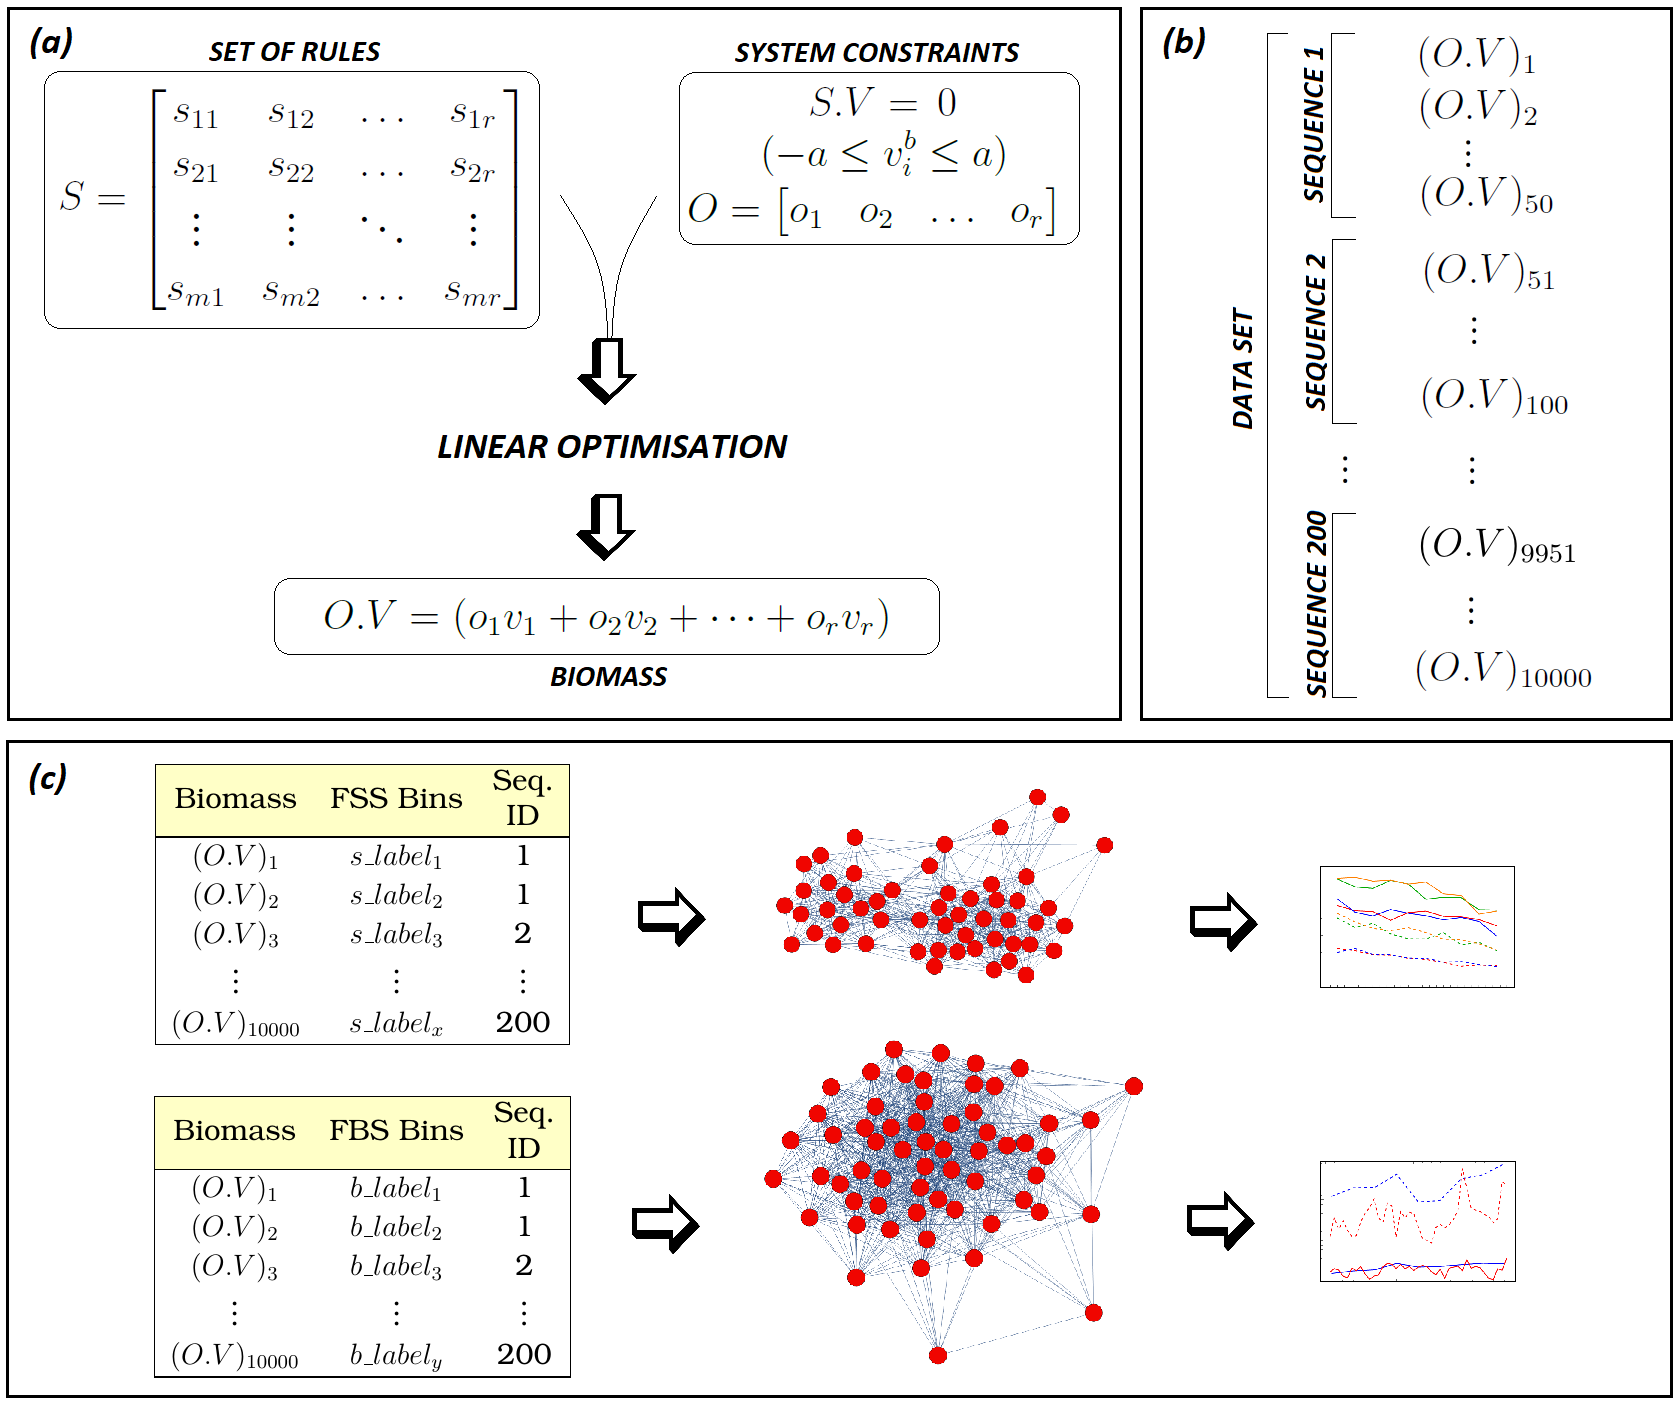
\includegraphics[width=1\linewidth]{../images/methodology-ORmodel-cartoon_complete_framework.png}}
		\caption{Simulation Model Illustration}
		\label{figure-complete_framework_cartoon}
	\end{center}
\end{figure}

%\begin{table}[hb!]
%	\centering
%	\setlength{\arrayrulewidth}{0.5pt}% 
%	\begin{tabular}{|ccc|}
%		\hline \rowcolor[HTML]{FFFFC7}
%		Biomass & FSS Bins	& \makecell{Seq.\\ID}  	\\ \hline
%		$(O.V)_{1}$	    & $s\_label_{1}$	& 1 		\\
%		$(O.V)_{2}$	    & $s\_label_{2}$	& 1 		\\
%		$(O.V)_{3}$	    & $s\_label_{3}$	& 2 		\\
%		\vdots  		& \vdots		& \vdots 	\\
%		$(O.V)_{10000}$	& $s\_label_{x}$	& 200 		\\ \hline
%	\end{tabular}
%\end{table}
%\begin{table}[hb!]
%	\centering
%	\setlength{\arrayrulewidth}{0.5pt}% 
%	\begin{tabular}{|ccc|}
%		\hline \rowcolor[HTML]{FFFFC7}
%		Biomass & FBS Bins	& \makecell{Seq.\\ID}  	\\ \hline
%		$(O.V)_{1}$	    & $b\_label_{1}$	& 1 		\\
%		$(O.V)_{2}$	    & $b\_label_{2}$	& 1 		\\
%		$(O.V)_{3}$	    & $b\_label_{3}$	& 2 		\\
%		\vdots  		& \vdots		& \vdots 	\\
%		$(O.V)_{10000}$	& $b\_label_{y}$	& 200 		\\ \hline
%	\end{tabular}
%\end{table}

%\begin{equation} %\tag{8}
%	(O.V)_{1}= (o_{1,1}v_{1} + o_{1,2}v_{2} + \dots + o_{1,r}v_{r})
%\end{equation}

%\begin{equation} %\tag{8}
%	(O.V)_{2}= (o_{2,1}v_{1} + o_{2,2}v_{2} + \dots + o_{2,r}v_{r})
%\end{equation}

%\begin{equation} 	
%	(O.V)_{50}= (o_{50,1}v_{1} + o_{50,2}v_{2} + \dots + o_{50,r}v_{r})
%\end{equation}

%\begin{equation} 	
%	(O.V)_{51}= (o_{1,1}v_{1} + o_{1,2}v_{2} + \dots + o_{1,r}v_{r})
%\end{equation}

%\begin{equation} 	
%	(O.V)_{100}= (o_{50,1}v_{1} + o_{50,2}v_{2} + \dots + o_{50,r}v_{r})
%\end{equation}

%\begin{equation} 	
%	(O.V)_{10000}= (o_{50,1}v_{1} + o_{50,2}v_{2} + \dots + o_{50,r}v_{r})
%\end{equation}

{\color{red} 
	An event is a single run of my optimization algorithm.
	
	The association network data sets were structured by the dot products of objective function vectors and optimized solution vectors. This product results maximize the output, as the maximization attempt of biomass in the FBA model.
	
	Explain how we introduce production sequence concept for the FBA.
	
	Network step sizes were always kept between $40$ and $50$.
}
